\chapter{oldapproach} % Main chapter title

\label{Chapter3} % For referencing the chapter elsewhere, use \ref{Chapter1} 

\lhead{Chapter 3. \emph{oldapproach}}


\section{Selenium Tests}
\label{sec:WritingTests}
\begin{verbatim}
Which is the best locator among ID, ID+LinkText, XPath and XPath+LinkText in terms of maintenance cost reduction?
In other words, we are interested to determine whether one (or more) of the proposed methods for locating UI elements is clearly better than the other ones for reducing the effort to
repair a test suite when a new version of a WAUT is created. We measured the dependent variable repairing effort in terms of time (minutes) and number of line of code to change for all the four considered test suites.
\end{verbatim}
\vspace{-2mm} The first phase of our approach involves writing Java-coded Selenium tests for the chosen reference versions of the AUT. Furthermore, in case of web applications having existing Selenium test-suites available for reasonable number of versions, we intend to leverage such tests for our analysis. Our approach treats the AUT as a black-box and executes system level tests using Selenium WebDriver framework. To improve the quality and maintainability of the tests, we aim to write modular Selenium tests adhering to the Page-Object pattern. To improve the stability of the tests, we intend to use attributes such as element-ID, name or CSS-selectors for detecting the GUI elements. In case of unavailability of these parameters, we may resort to detecting the elements using XPath or link text locators. 

During the development of the Selenium tests, we aim to locally execute and test them.  By employing these tests, we intend to cover the core application functionalities of the AUT. We intend to perform our experiment on 4-5 different web application subjects, preferably open-source. We intend to include the subjects from different domains along with sufficient number of major versions (3-5) and minor revisions/commits. We intend to include 3-5 applications in our set of experimental subjects, for which existing Selenium tests are available for usage. Moreover, to verify our approach during the initial stages we might include a relatively small scaled application subject.

\section{Generating Behavioral State Models}
\label{sec:BehavModels}

\vspace{-2mm}
Subsequently, in the second phase we plan to integrate these tests with \textit{WebMate} in order to identify the behavioral and GUI state level differences between the reference version and the subsequent versions of the AUT. In order to expedite this process, we aim to deploy multiple versions of the AUT in parallel, on a remote server such as a Linux based virtual machine. Figure  \ref{fig:deployment} depicts the overview of remote automatic deployment process; three versions of the AUT are running simultaneously against their individual database instances. The general test set-up to concurrently and independently execute tests across these versions and to extract behavioral state models is as depicted in figure \ref{fig:stateModelExtraction}.  \textit{WebMate} takes the Selenium test suite and the application’s base URL as input and executes the tests on different versions of the AUT to generate the behavioral state models. Afterwards we plan to detect the GUI level differences across these versions using \textit{WebMate}. During this phase, we provide \textit{WebMate} with the URLs for different application states as input. As output, \textit{WebMate} highlights the changed and/or missing GUI elements for different versions in comparison to the reference version of the AUT. Thereafter, we intend to map the behavioral state differences to GUI level differences to confirm whether changing active GUI elements (e.g. clickable fields, buttons) have manifested a changed application behavior.

\begin{figure}[h!]
\makeatletter 
\renewcommand{\thefigure}{\@arabic\c@figure}
\makeatother
    \centering
  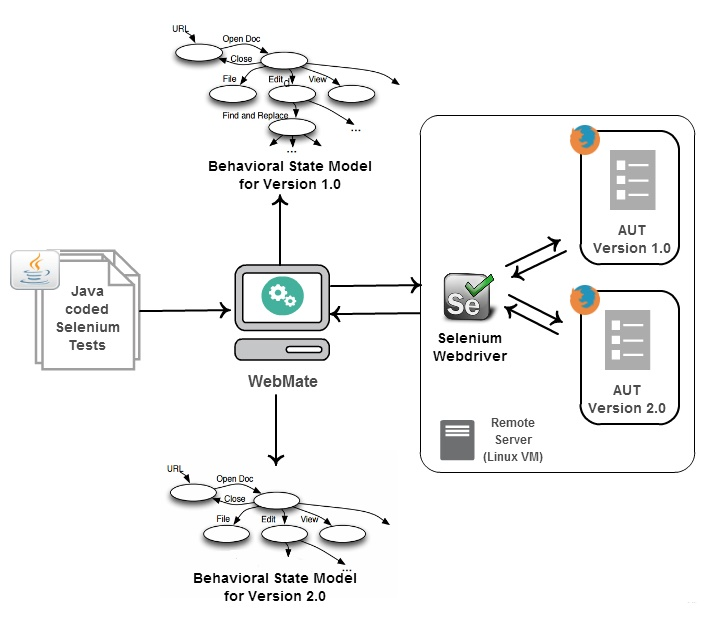
\includegraphics[width=5in,height=4in]{./Figures/WebMate_state_extraction}
  \caption{Extraction of behavioral state models using WebMate \cite{webmate}}
  \label{fig:stateModelExtraction} 
\end{figure}

\section{Measuring the Robustness Metric}
\label{sec:MeasureRobMetric}
\vspace{-2mm} To measure the robustness metric, we perform pair-wise equivalence check of the reference and test versions to assess whether same application states are covered. For cases where all the states are matched, robustness metric of given test-suite is 100\%. We propose to distribute the behavioral model generation and robustness measurement across the major and minor versions of the AUT, as mentioned in Section


\begin{center}
\begin{scriptsize}
\centering
\lstset{
  basicstyle=\ttfamily,
  columns=fullflexible,
  keepspaces=true,
%   frame=none,
}
% \verb|basicstyle=\ttfamily, columns=fullflexible, keepspaces=true|
  
\begin{lstlisting}[caption=Page-Objects design for \texttt{loginTest},label=code2]
actions : { 
[session-Id, get {url="http://application-under-test.com"}]
},
 actions : { 
[session-Id, findElement {using="id", value="username"}]
},
 actions : { 
[session-Id, sendKeysToElement {id="1", value=["uname"]}],
[session-Id, findElement {using="id", value="password"}]
},
 actions : { 
[session-Id, sendKeysToElement {id="2", value=["MOODLE_admin_121"]}],
[session-Id, findElement {using="link text", value="Login"}]
},
 actions : { 
[session-Id, clickElement {id="3"}]
}
\end{lstlisting}
\end{scriptsize} 
\end{center}


% Selenium tests might not be fully robust if they cover the intended behavior for the reference version but fail to cover the same behavior for subsequent test versions. Test failures can be detected by using assertions in the code, analyzing test reports, verifying that the application is in the intended state by capturing the screen-shots, finite state models for the application state etc. While useful, these techniques suffer certain drawbacks such as investment of time as well as manual efforts required for the analysis of their outcome. Approaches involving screenshot comparison might not be able to fully reveal the covered behavior and unexplored functionalities. Although finite state models can detect the covered functionalities, current implementations do not evaluate and compare these models for functional changes across different versions of an application. 

% In the area of leveraging existing Selenium tests and generating behavioral models, the 'Testilizer' project by Mesbah et al \cite{testilizer} implements the combination of manual and automated test generation by leveraging manual tests with automated crawling. This approach focuses on mining the human-written tests to explore additional application functionality which might be unexplored by the crawler. It implements strict automatic assertion generation and as a result, the exploration depth to cover available functionality is limited. Another approach by Mesbah and Prasad \cite{CBCMesbah} proposes behavioral and functional differential analysis in the area of cross-browser compatibility; however it inherits the drawbacks suffered by 'Testilizer' such as limited recursion depth and additional effort required to identify active GUI elements. Another approach to cross-browser testing involves ‘WebDiff’ by Choudhary et al \cite{WebDiff} which implements DOM-tree matching and pair wise screen-shot comparison to detect cross browser issues. Our approach leverages the principles behind cross-browser analysis and applies the techniques such as functional and GUI-level differential analysis to differentiate the behavioral coverage achieved by Selenium tests across different versions of the AUT.

% As a comparative study of maintainability of Selenium WebDriver test-suites, Leotta et al \cite{leotta2013comparing} propose an approach to analyze the effectiveness and failure of Selenium tests on the basis of Element-locators. Their approach limits the analysis to a comparative study of element locators and does not consider other factors mentioned in Section \ref{sec:RobustnessFactors} responsible for the instability of Selenium tests. 

% Considering the current state-of-the-art technologies to our knowledge, there are no similar approaches to implement the robustness analysis of Selenium tests. Moreover, none of the aforementioned approaches evaluates the robustness of Selenium test-suites over the version history of the AUT. In contrast, our approach incorporates the existing techniques such as behavioral state models and GUI level comparisons to evaluate the robustness of Selenium tests and investigates the test failures across different regression cycles.